\subsection{BMS}
\label{subsec:bms-monitor}
% monitor bms display led and sit down when empty
% speaker usage? battery low

Nutzt man den \gls{go1} im Batterie-Betrieb, so sollte man stets darauf achten, dass die Ladung des Akkus nicht unter
\num{3} \% fällt, da die Motoren bei diesem Ladestand zur Sicherheit abgeschaltet werden.
Die Umsetzung des Entwicklerteams der Firma Unitree hat in diese Sicherheitsfunktion jedoch wenig Arbeit investiert.
So ist die einzige ständig sichtbare Anzeige der Akkuladung außen am Akku angebracht und nur von einer Seite einsehbar.
Zudem kann die Anzeige die Ladung nur in acht Schritten anzeigen und ist somit nicht genau genug.
Auch das abrupte Abschalten der Motoren ist potenziell schädlich für den Roboter, da dieser nicht zuerst in einen liegenden
Zustand gebracht wird, was zur Folge haben kann, dass er in jeder erdenkbaren Position zusammensackt.
Die einzelnen Glieder der vier Beine und der Rumpf fallen dann ungeschützt und prallen auf dem Boden auf.

Um diesem Mangel entgegenzusetzen und den Roboter somit resilienter gegen vermeidbare Schäden zu machen, wird in diesem
Kapitel ein Batterie-Monitoring-System mit aktiver Warnung und vorsichtiger Motorabschaltung implementiert.
Ziel ist es, bei einer niedrigen Akkuladung von \num{5} \% eine Warnung über die \glspl{led} des Kopfes darzustellen und den
\gls{go1} dann sanft zu Boden zu lassen, bevor die eingebauten Mechanismen bei \num{3} \% Ladung greifen und die Motoren
abschalten.
Hierfür werden die bereits verbauten Funktionen MQTT und Autostart verwendet.
Dokumentation hierfür sind im Kapitel \ref{subsec:funktionen} zu finden.

\myparagraph{Entwurf}

Abbildung \ref{fig:sequenz-bms} zeigt das Sequenzdiagramm zur Darstellung des Batterie-Monitorings.

\begin{figure}[h]
    \frame{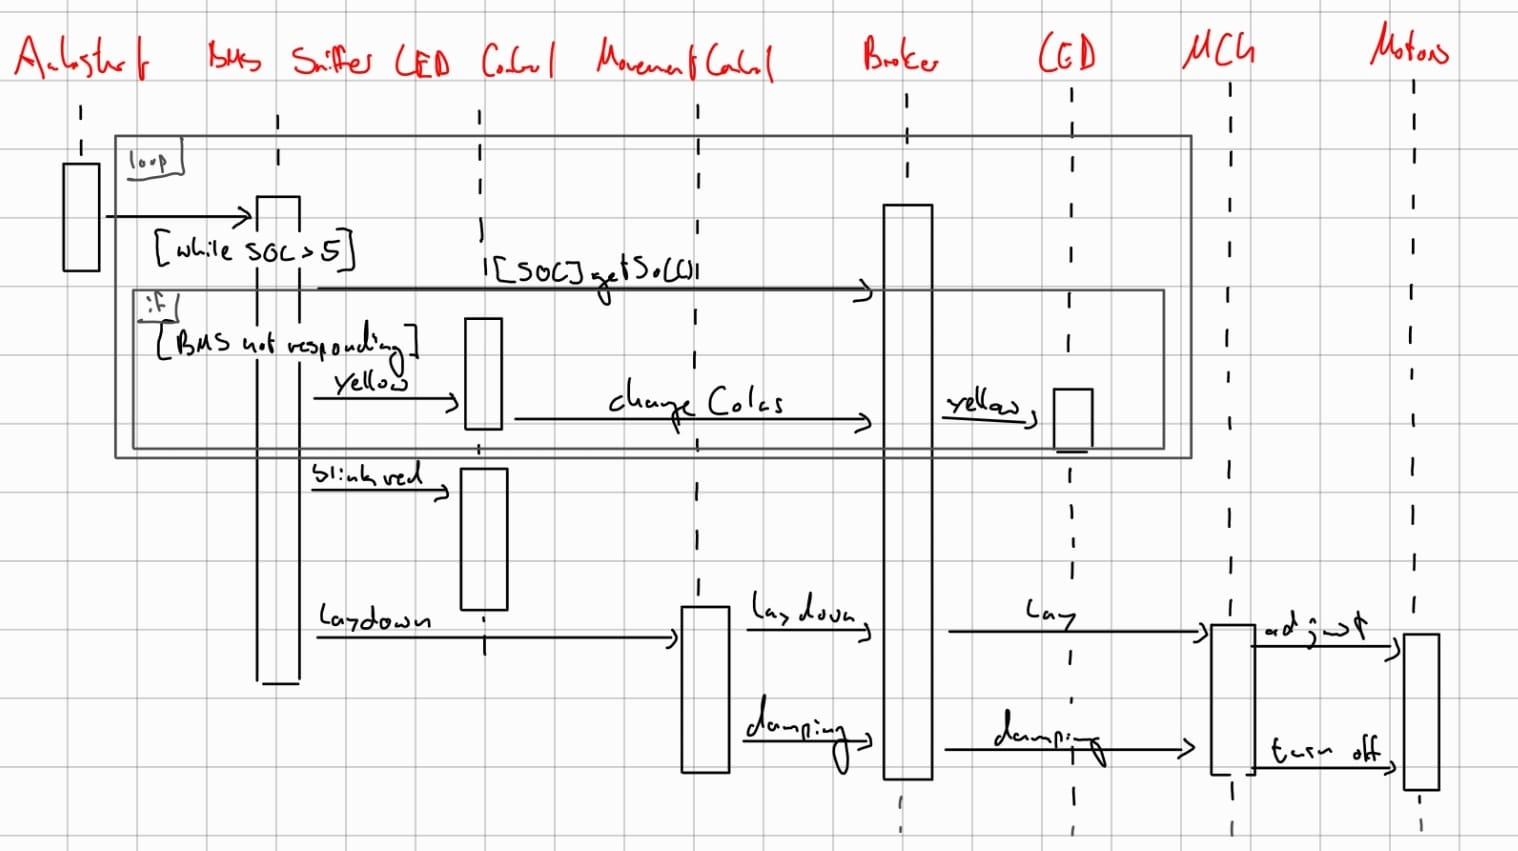
\includegraphics[width=\linewidth]{img/erweiterung/sequenz-bms}}
    \caption{Sequenzdiagramm der Batterie-Monitoring Komponenten}\label{fig:sequenz-bms}
\end{figure}

\noindent Die beteiligten Komponenten des Roboters sind die Autostart-Funktion, die Software-Komponenten BMS-Sniffer, LED-Control
und Movement-Control, der MQTT-Broker, die \glspl{led} des Kopfes, die \gls{mcu} und die zwölf Motoren.
Tatsächlich interagiert wird lediglich mit der Autostart-Funktion und dem MQTT-Broker, die drei Software-Komponenten müssen
noch entwickelt werden.

Das Autostart-Modul auf dem Raspberry Pi soll um die neue Funktionalität \texttt{bmsMonitoring} erweitert werden.
Hierfür wird ein Ordner mit Skript angelegt, das alle weiteren Software-Komponenten auslöst.
Das Modul BMS-Sniffer soll dauerhaft die \gls{bms} Daten über den MQTT-Broker abfragen.
Ist das \gls{bms} nicht erreichbar, beispielsweise weil der Roboter im Netzbetrieb ohne Akku gestartet wurde,
so wird die Komponente LED-Control aufgerufen, welche die \glspl{led} des Roboters dauerhaft gelb leuchten lässt.
Sollte das \gls{bms} erreichbar sein und die \gls{soc} auf \num{5} \% oder weniger fallen, so wird zuerst LED-Control
aufgerufen, um die \glspl{led} des \gls{go1} rot blinken zu lassen, worauf das Movement-Control-Modul aufgerufen wird,
um den Roboter erst hinzulegen und danach die Motoren zu entspannen (Damping-State).
Sowohl das LED-Control-Modul als auch das Movement-Control-Modul nutzen den MQTT-Broker als Schnittstelle zu den zu steuernden
Hardwarekomponenten.

\myparagraph{Umsetzung}

Für die Umsetzung des \gls{bms}-Monitors muss zuerst die Autostart-Funktion ergänzt werden.
Hierfür muss der Ordner \texttt{/home/\allowbreak pi/\allowbreak Unitree/\allowbreak autostart/\allowbreak bmsMonitor}
erstellt werden.
In diesem wird das Skript \texttt{bmsMonitor.sh} angelegt, welches lediglich ein weiteres Skript namens \texttt{run.sh}
als Hintergrundprozess startet.
Dieser Schritt ist nötig, um die Monitoring-Funktion vom Autostart-Prozess zu entkoppeln.
Das \texttt{run.sh} Skript startet nun alle Loggingaktivitäten und die nötigen Software-Komponenten.
Als letzter Schritt muss die neue Funktion noch in die Startup-Liste
\texttt{/home/pi/Unitree/autostart/.startlist.sh}
angehängt werden.

Um die Entwicklung und Anpassung der Autostart-Funktion zu vereinfachen, kann der Quellcode in einem Ordner an anderer
Stelle über die Versionsverwaltung \emph{Git} aktuell gehalten werden.
Die einzelnen Dateien und Ordner können über ein Installationsskript in die Autostart-Funktion integriert werden.
Folgendes Listing zeigt die relevanten Teile des Installationsskriptes.
Die vollständigen Dateien sind im Anhang zu finden.

\lstinputlisting[language=Bash,numbers=left,xleftmargin=\dimexpr2.5em-1pt,framexleftmargin=2em,firstline=33,lastline=40,firstnumber=33]{listing/go1-bmsMonitor/install.sh}

\noindent Folgende Übersicht zeigt den Aufbau des Quellcode-Ordners zur Einordnung des Installationsskripts und der weiteren Erklärungen.

\vspace*{5pt}
\dirtree{%
    .1 go1-bmsMonitor.
    .2 bmsMonitor.
    .3 bmsMonitor.sh.
    .3 constants.sh.
    .3 led\_control.py.
    .3 requirements.txt.
    .3 run.sh.
    .3 sniff\_bms.py.
    .2 install.sh.
}

Der eigentliche Einstieg des \texttt{bmsMonitor} ist die Datei \texttt{run.sh}, die als Hintergrundprozess durch den
Autostart gestartet wird.
Diese installiert vorerst alle benötigten \emph{Python}-Bibliotheken, die in der \texttt{requirements.txt} Datei hinterlegt
sind.
Daraufhin wird das Skript \texttt{sniff\_bms.py} gestartet, welches den BMS-Monitor enthält.

\lstinputlisting[language=Bash,numbers=left,xleftmargin=\dimexpr2.5em-1pt,framexleftmargin=2em,firstline=8,lastline=9,firstnumber=8]{listing/go1-bmsMonitor/bmsMonitor/run.sh}

\noindent Die Zeilen \num{13} bis \num{23} des Skripts \texttt{sniff\_bms.py} zeigen die Umwandlung der binären Message-Payload
bei neuen MQTT-Nachrichten und die weitere Auswertung der \gls{soc}.

\lstinputlisting[language=Bash,numbers=left,xleftmargin=\dimexpr2.5em-1pt,framexleftmargin=2em,firstline=13,lastline=23,firstnumber=13]{listing/go1-bmsMonitor/bmsMonitor/sniff_bms.py}

\noindent Die Methode \texttt{struct.unpack(...)} zeigt die in Kapitel \ref{subsubsec:batterie-management} erarbeitete
Dekodierung der Message-Payload des Topics \texttt{bms/state}.
In Zeile \num{19} wird geprüft, ob das \gls{bms} aktiv ist.
Ist das \gls{bms} inaktiv, so besteht die Message-Payload nur aus binären Nullen.
In diesem Fall wird die Funktion \texttt{const\_led(c,r,g,b)} aus dem Modul LED-Control in der Datei \texttt{led\_control.py}
aufgerufen.

\lstinputlisting[language=Bash,numbers=left,xleftmargin=\dimexpr2.5em-1pt,framexleftmargin=2em,firstline=14,lastline=16,firstnumber=14]{listing/go1-bmsMonitor/bmsMonitor/led_control.py}

\noindent Die Übergabeparameter \texttt{r}, \texttt{g} und \texttt{b} sind die RGB-Werte, die die \glspl{led} am Kopf des
Roboters annehmen sollen.
Der Parameter \texttt{c} ist die MQTT-Client-Instanz, die zur Kommunikation mit dem Broker genutzt wird.
Das Format des MQTT-Topics \texttt{face\_light/color} ist in Kapitel \ref{subsubsec:led} beschrieben.
Die RGB-Werte \texttt{r=10}, \texttt{g=10} und \texttt{b=0} stellen die \glspl{led} auf ein sehr gedimmtes Gelb ein.

In Zeile \num{21} der Datei \texttt{sniff\_bms.py} prüft den Wert des \gls{soc} des Akkus, ist dieser größer als \num{5},
so endet die Funktion und es wird auf die nächste MQTT-Nachricht gewartet.
Andernfalls werden die \glspl{led} in der \texttt{alert\_led.py} Funktion der Datei \texttt{led\_control.py}
auf Rot-blinkend konfiguriert.

\lstinputlisting[language=Bash,numbers=left,xleftmargin=\dimexpr2.5em-1pt,framexleftmargin=2em,firstline=7,lastline=11,firstnumber=7]{listing/go1-bmsMonitor/bmsMonitor/led_control.py}

\noindent Die Übergabeparameter sind hier die gleichen wie in der Funktion \texttt{const\_led(c,r,g,b)}.
Nur den Wert \texttt{r=255} zu setzen hat zur Folge, dass die \glspl{led} in der maximalen Helligkeit Rot leuchten.
Die Funktion \texttt{lay\_down()} des Moduls Movement-Control ist der Einfachheit wegen in der Datei \texttt{sniff\_bms.py}
formuliert.

\lstinputlisting[language=Bash,numbers=left,xleftmargin=\dimexpr2.5em-1pt,framexleftmargin=2em,firstline=31,lastline=33,firstnumber=31]{listing/go1-bmsMonitor/bmsMonitor/sniff_bms.py}

\noindent Die Funktion sendet lediglich zwei Befehle an das MQTT-Topic \texttt{controller/action}.
Die \texttt{action} \texttt{standDown} bewirkt, dass der Roboter alle vier Beine anwinkelt und somit den Rumpf nah an
den Boden bewegt.
Die \texttt{action} \texttt{damping} bewirkt, dass der Roboter die Spannung aus den Gelenken nimmt und die Motoren deaktiviert.
Das hat zur Folge, dass der Roboter leicht zusammensackt, weshalb er vorher hingelegt werden sollte.
Die gesamte Aktion der \gls{led} Konfiguration und des Hinlegens ist kurz genug, dass die \gls{soc} des Akkus nicht auf
\num{3} \% fällt.
Sobald dies passiert werden die Motoren abgeschaltet und können nicht mehr verwendet werden.
Die Konstanten der gesamten Python-Umgebung sind in der Datei \texttt{constants.py} hinterlegt.

\lstinputlisting[language=Bash,numbers=left,xleftmargin=\dimexpr2.5em-1pt,framexleftmargin=2em]{listing/go1-bmsMonitor/bmsMonitor/constants.py}
\todo{Breite der Box nicht wie lst env} % todo breite graue box lstinput und lst env nicht gleich

\noindent Zur finalen Installation der Erweiterung kann wie folgt vorgegangen werden.

\begin{lstlisting}[language=Bash]
pi@raspberrypi:~ $ mkdir ~/Extensions/ && cd ~/Extensions
pi@raspberrypi:~/Extensions $ git clone <Repository Link>
pi@raspberrypi:~/Extensions $ cd go1-bmsMonitor/
pi@raspberrypi:~/Extensions/go1-bmsMonitor $ sh install.sh
\end{lstlisting}

\noindent Das Installationsskript erstellt einen Link im Autostart-Ordner zum Verzeichnis des geklonten Git-Repositories und
konfiguriert die Skripte, sodass sie ausführbar sind.
Bei einem erneuten Systemstart des Raspberry Pi wird die Funktion am Ende des Autostart-Prozess' gestartet.
Der gesamte Quellcode kann in dem zur Versionsverwaltung angelegten Git-Repository genauer untersucht werden\footcite{git-bms-monitor}.
